\documentclass[preprint,12pt]{elsarticle}

\usepackage[T1]{fontenc}
\usepackage[utf8]{inputenc}
\usepackage{amsmath,amssymb,amsthm}
\usepackage{graphicx}
\usepackage{booktabs}
\usepackage{multirow}
\usepackage{placeins}
\usepackage{float}
\usepackage{algorithm}
\usepackage{algpseudocode}
\usepackage{hyperref}
\hypersetup{colorlinks=true,linkcolor=blue,citecolor=blue,urlcolor=blue}
\usepackage[capitalise,noabbrev]{cleveref}

\newtheorem{proposition}{Proposition}
\newtheorem{definition}{Definition}
\newtheorem{assumption}{Assumption}

\biboptions{numbers,sort&compress}

\journal{Engineering Applications of Artificial Intelligence}

\begin{document}

\begin{frontmatter}

\title{Alert-Budgeted Clinical Early Warning: Conformal Risk Control for Stateful Deterioration Alarm Policies}

\author[a]{First Author\corref{cor1}}
\ead{first.author@institution.edu}
\author[a]{Second Author}
\author[b]{Third Author}

\cortext[cor1]{Corresponding author.}

\affiliation[a]{organization={Department, Institution}, city={City}, postcode={000000}, country={Country}}
\affiliation[b]{organization={Department, Institution}, city={City}, postcode={000000}, country={Country}}

\begin{abstract}
Clinical early warning systems are evaluated almost exclusively by discrimination, yet their failure in deployment is operational rather than statistical: intensive care units generate alarm volumes far beyond what clinical staff can absorb, and the resulting alarm fatigue erodes the very safety the systems are meant to provide. This paper treats the alarm budget, defined as the tolerated number of alarms per patient-day, as a first-class design constraint rather than a post hoc threshold adjustment. We formalise early warning as a stateful alarm policy whose refractory window and escalation tier are explicit control variables, and we show that the resulting temporal dependence invalidates timestep-level conformal calibration. We therefore develop a patient-level blocked conformal risk control procedure that restores finite-sample validity for dependent alarm sequences and yields an upper bound on the probability that the deployed population alarm rate exceeds the operational budget. The method is instantiated on irregularly sampled intensive care trajectories using two open, multi-hospital cohorts, and is evaluated under cross-hospital transfer, prevalence shift, and observation sparsification. The AI contribution is a calibration procedure that provides distribution-free control of alarm rate for policies with internal state; the engineering contribution is an operating-point selection mechanism that lets a monitoring system be specified by its alarm budget and then certified against it. The evaluation protocol compares all methods at matched alarm budgets rather than at matched thresholds, reports detection lead time and net benefit alongside discrimination, and quantifies the empirical budget violation rate over repeated calibration splits.

\end{abstract}

\begin{keyword}
Clinical early warning \sep Clinical deterioration \sep Alarm fatigue \sep Conformal prediction \sep Irregularly sampled time series \sep Decision support systems
\end{keyword}

\end{frontmatter}

\section{Introduction}
\label{sec:intro}

Deterioration events in hospitalised patients unfold over hours, and the physiological trajectory that precedes them is recorded long before the event itself is recognised. This temporal structure has motivated a substantial literature on data-driven early warning, ranging from static severity scores to sequential models that forecast deterioration trajectories from electronic health records \citep{xiumin2026machine} and compact, efficiency-aware networks that predict sepsis onset from structured time series \citep{taparugssanagorn2026lightweight}. Reported discrimination is high and improving, with in-hospital mortality and onset prediction now routinely exceeding the performance of classical scoring instruments \citep{yong2024deep}. The implicit promise of this line of work is that a sufficiently accurate model, once installed at the bedside, will shorten time to intervention.

Discriminative prediction and operational alerting address different questions. A score-to-alert conversion requires a decision rule, whereas threshold-independent ranking metrics do not specify how frequently that rule emits alarms. Reviews of intensive-care adverse-event prediction discuss incomplete reporting of alert burden, time-to-alert and deployment calibration \citep{wang2026deep}. Reviews of multivariate clinical time-series learning also motivate evaluation beyond architectural comparisons \citep{hernandezdiaz2026deep,swinckels2024deep}. These concerns support reporting the alarm policy and its realised load explicitly, rather than treating an area-under-the-curve comparison as a specification of bedside alerting behaviour.

Recent research improves the backbone that produces the risk score. For irregularly sampled and heterogeneously missing observations, approaches include reliability-aware temporal aggregation \citep{kim2026retamamba,shen2026enhancing}, graph formulations over irregular observations \citep{yalavarthi2024grafiti}, and masked-attention models for deterioration prediction \citep{mun2026made}. Transfer-oriented variants align feature spaces across cohorts \citep{komolafe2025early}, while dynamic temporal graphs incorporate clinical calculators into the prediction pathway \citep{yin2024sepsiscalc}. These methods motivate prospective backbone comparisons, but their adapters are not included in the current reference implementation. Our implemented contribution instead concerns the causal mapping from fixed scores to stateful alarms and the risk associated with selecting that mapping.

A separate literature attaches reliability estimates to clinical predictions. Selective prediction and calibration have been analysed for multimodal clinical classification \citep{lpez2026empirical}, reliability estimation has been extended beyond output-space calibration for time-series classifiers \citep{cenacchi2026beyond}, and conformal methods have been used for physiological regression uncertainty \citep{strickland2025degrees}. Our distinction is the unit and estimand of alarm-policy calibration: refractory state makes successive emitted alarms dependent, so those hours cannot simply be counted as independent patient samples. This does not imply that every conformal treatment of time series is invalid or that a stateful policy cannot be calibrated at the trajectory level. The reference construction uses independent patient blocks and fixed finite-grid upper-confidence bounds, a stronger sampling assumption than exchangeability alone.

This draft makes the alarm budget an explicit constraint and calibrates the policy that generates alerts. The implementation separates causal score estimation from full-trajectory policy replay. Its finite-sample bound concerns the population mean of patient-level rates, not a hard maximum for each patient or ward. Real-cohort comparisons remain prospective, and the current contributions are as follows.
\begin{itemize}
\item We formulate early warning as a stateful alarm policy in which the refractory window and escalation tier are control variables, so that alarm volume becomes a design parameter of the monitoring system rather than an emergent property of a threshold.
\item We derive a patient-blocked finite-grid upper-confidence bound on the population alarm rate under independent sampling, and distinguish it from a deliberately invalid timestep effective-sample-size shortcut.
\item We provide causal reference learners and official-format data readers, and specify a prospective evaluation protocol under shared requested budgets, with cross-hospital transfer and observation sparsification as planned extensions.
\end{itemize}
The remainder of the paper reviews related work (\cref{sec:related}), develops the policy formulation and the calibration procedure (\cref{sec:method}), and specifies the datasets, baselines, metrics, and experimental protocol (\cref{sec:setup}).

\section{Related Work}
\label{sec:related}

\subsection{Backbones for Irregularly Sampled Clinical Time Series}

The modelling substrate for early warning is a sequence of observations whose sampling times carry as much information as their values. The most recent work in this line treats irregularity as a first-class object rather than an inconvenience: continuous-time formulations parameterise the latent trajectory between observations and evaluate it at arbitrary query times \citep{shen2026enhancing}, reliability-aware aggregation weights observations by their estimated trustworthiness before temporal pooling \citep{kim2026retamamba}, and graph constructions connect observations across variables and time so that forecasting can propagate information along non-uniform edges \citep{yalavarthi2024grafiti}. A complementary strand models the observation process itself, on the argument that the decision to order a laboratory test is a clinical action and therefore informative; this idea has been used both to synthesise realistic irregular trajectories \citep{mehdizavareh2026informative} and to build masked-attention predictors for deterioration on general wards \citep{mun2026made}. Domain-specific instantiations extend the same machinery to data-scarce settings such as venous thromboembolism detection after cancer treatment \citep{xu2026bridging}, and surveys of the area converge on the observation that architectural progress has outpaced agreement on evaluation \citep{sun2026review}. We adopt these backbones without modification and treat the score function they produce as an input to our policy layer, which is where our contribution lies.

\subsection{Early Warning and Deterioration Prediction}

Clinical early warning has moved from static severity scores toward dynamic, trajectory-aware prediction. Recent multicentre work predicts the shape of sepsis deterioration rather than a single risk estimate, arguing that heterogeneous trajectories require patient-specific forecasting \citep{xiumin2026machine}, while efficiency-oriented designs pursue compact models that remain explainable under the compute constraints of a ward workstation \citep{taparugssanagorn2026lightweight}. Others inject clinical reasoning into the prediction pathway: dynamic temporal graphs embed calculator-derived features so that the model inherits the semantics of established instruments \citep{yin2024sepsiscalc}, and language-model-guided simulation is used to generate interpretable physiological dynamics for early warning \citep{nie2026clinically}. Transfer-oriented formulations address the practical reality that a model trained in one institution must be reused in another with different coding practice and case mix \citep{komolafe2025early}, and earlier work established that deep models over longitudinal inpatient records can outperform tabular baselines for outcome prediction \citep{rong2025deep,yong2024deep,mohammad2024early}. Across this literature the model is the unit of contribution; the alerting rule that converts its output into an operational signal is treated as an afterthought, and comparison between methods is almost always conducted at a fixed threshold rather than at a fixed alarm volume.

\subsection{Calibration, Selective Prediction, and Conformal Guarantees}

A parallel literature asks not whether a model is accurate but whether its outputs can be trusted at a stated level. Systematic analysis of calibration and selective prediction for multimodal clinical classification shows that abstention behaviour, not raw discrimination, determines whether a system is safe to deploy \citep{lpez2026empirical}. For time-series classifiers, reliability estimation has been extended beyond post hoc remapping of output scores toward evidence that a confident prediction is actually supported by the input \citep{cenacchi2026beyond}, and audits of adaptation procedures have exposed failure modes that only appear when the update rule is evaluated with realistic label delays \citep{fentazi2026training}. Conformal prediction supplies the distribution-free coverage guarantee that these approaches seek, and has been applied to physiological regression where calibrated uncertainty is a safety requirement \citep{strickland2025degrees}. Adaptation at inference time has also been used to counter patient-specific shift in haemodynamic prediction \citep{li2026crosssample}. What this body of work assumes, and what an operational alarm system violates, is independence: a decision rule with a refractory period produces a dependent sequence, so guarantees derived from exchangeable examples do not transfer to the alarm rate actually experienced by a clinical unit. Our procedure is designed for exactly this dependent regime.

\subsection{Evaluation Practice}

Finally, the reporting conventions of the field shape what gets optimised. Risk-of-bias instruments for prediction models have recently been extended to cover artificial-intelligence-specific failure modes, including the handling of calibration, heterogeneity, and operational applicability \citep{moons2025probastai}, and methodological reviews of intensive-care adverse-event prediction note that alert burden and time-to-alert remain inconsistently reported \citep{wang2026deep,hernandezdiaz2026deep,swinckels2024deep}. We take these critiques as a specification: every experiment below reports an operational quantity alongside a statistical one, and all comparisons between alerting strategies are conducted at matched alarm budgets so that discrimination is never bought with unreported alarm volume.

\section{Method}
\label{sec:method}

\subsection{Problem Setting and Notation}

Let patient $i$ contribute an observation set $\mathcal{O}_i=\{(t_{ij},m_{ij},v_{ij})\}_{j=1}^{n_i}$ with observation times $t_{ij}\in[0,T_i]$, variable indices $m_{ij}\in\{1,\dots,d\}$, and values $v_{ij}\in\mathbb{R}$. The set is irregular in the sense that neither the number of observations nor their spacing is controlled by the analyst: a laboratory panel may be drawn four times in an hour and then not for eight hours. A score function $f_\theta$ maps the history available at time $t$, denoted $\mathcal{O}_{i,\le t}$, to a risk score $s_{it}=f_\theta(\mathcal{O}_{i,\le t})\in(0,1)$. The score function is treated as a black box in this section; any of the backbones in \cref{sec:related} may be substituted, and \cref{sec:setup} fixes a small set for the experiments.

The event of interest occurs at time $t^\star_i$, and for patients who never experience it we set $t^\star_i=\infty$. A prediction is useful if it fires in the window $[t^\star_i-W,\,t^\star_i)$ for a lead-time window $W$, which we fix at twelve hours following common practice in deterioration prediction. Because the score is defined at observation times only, all decisions below are indexed by the observation grid of each patient rather than by a global clock.

\subsection{Stateful Alarm Policies}

A threshold rule declares an alarm whenever $s_{it}\ge\lambda$. Such a rule has no memory, and in deployment it fires repeatedly on the same deteriorating patient, which is the mechanism by which alert volume becomes unmanageable. We therefore define an alarm policy $\pi_\lambda=(\lambda,\tau,\kappa)$ with three components: a threshold $\lambda$, a refractory window $\tau$ expressed in observation steps, and an escalation tier $\kappa$ that specifies how many suppressed exceedances must accumulate before the refractory period is overridden. The policy carries an internal state $z_{it}$ and emits
\begin{equation}
\label{eq:policy}
a_{it}=\mathbb{1}\!\left[s_{it}\ge\lambda \ \wedge\ \left(z_{it}=0 \ \vee\ c_{it}\ge\kappa\right)\right],
\qquad
z_{i,t+1}=
\begin{cases}
\tau, & a_{it}=1,\\
\max(0,\,z_{it}-1), & a_{it}=0,
\end{cases}
\end{equation}
where $c_{it}$ counts consecutive exceedances of $\lambda$ that were suppressed. The refractory window is the control that directly trades alarm volume against repeated detection, and the escalation tier prevents a long refractory period from masking a genuinely escalating patient. Setting $\tau=0$ and $\kappa=\infty$ recovers the memoryless threshold rule, so \cref{eq:policy} is a strict generalisation rather than a replacement.

Two properties of \cref{eq:policy} matter for what follows. First, the policy is a deterministic function of the score trajectory given $(\lambda,\tau,\kappa)$, so the only quantity that must be calibrated against deployment data is the scalar $\lambda$; the structural parameters are selected by cross-validation on the source cohort. Second, the emitted sequence $\{a_{it}\}$ is dependent in time by construction, and this dependence is not a nuisance to be averaged away but the mechanism through which the budget is enforced.

\subsection{Why Timestep-Level Calibration Fails}

It is tempting to calibrate $\lambda$ by treating each observation time as an example and applying split conformal prediction to the indicator $a_{it}$. This is invalid for two distinct reasons, and separating them clarifies what the proposed procedure must repair.

The first is granularity. The operational quantity is a rate per patient-day,
\begin{equation}
\label{eq:risk}
R(\lambda)=\mathbb{E}\!\left[\frac{1}{D_i}\sum_{t}a_{it}(\lambda)\right],
\end{equation}
where $D_i$ is the length of patient $i$'s record in days. The expectation is over patients, while the inner sum is over dependent observations. Controlling the marginal alarm probability at a randomly chosen timestep does not control \cref{eq:risk}: the two differ by the inverse of the mean record length and by the within-patient correlation of $a_{it}$.

The second is state dependence. Because $a_{it}$ depends on $a_{i,t-1}$ through $z_{it}$, the timestep-level losses are neither independent nor exchangeable once the policy is active. Calibrating on a pooled timestep sample therefore estimates the alarm rate of a policy evaluated on a different dependence structure from the one that will run in the ward. The error is not conservative in either direction; it depends on how strongly alarms cluster, which is precisely the regime a well-designed refractory window creates.

\subsection{Blocked Conformal Risk Control}

The repair is to move the unit of calibration from the timestep to the patient. Define the patient-level loss
\begin{equation}
\label{eq:blockloss}
L_i(\lambda)=\frac{1}{D_i}\sum_{t}a_{it}(\lambda)\in[0,\,L_{\max}],
\end{equation}
which is exactly the quantity inside the expectation in \cref{eq:risk}. The bound is $L_{\max}=\sup_{H\ge H_{\min}}\frac{24}{H}\left(\left\lfloor\frac{H/\Delta-1}{\tau+1}\right\rfloor+1\right)$, where $H$ is the length of stay, $\Delta$ the sampling interval and $H_{\min}$ the shortest stay admitted to the cohort. The supremum is not attained at one day: with hourly sampling and $\tau=4$ a 26-hour stay permits six alarms, or $144/26\approx5.54$ per day, while a 24-hour stay permits only five. Evaluating the bound at a nominal day therefore understates it, and since short stays are exactly the ones that generate high per-day rates, $H_{\min}$ is a modelling decision that must be declared rather than a detail. Patients are exchangeable draws from the deployment population even though observations within a patient are not, so averaging \cref{eq:blockloss} over patients restores the exchangeability that conformal calibration requires. Let $\Lambda$ be a finite grid of candidate thresholds and let $\widehat{R}_n(\lambda)=\frac{1}{n}\sum_{i=1}^{n}L_i(\lambda)$ be the calibration average over $n$ held-out patients.

\begin{proposition}[Budget validity]
\label{prop:validity}
Fix $\alpha\in(0,1)$ and a budget $B>0$. Let
\begin{equation}
\label{eq:lambda}
\widehat{\lambda}=\inf\left\{\lambda\in\Lambda:\ \widehat{R}_n(\lambda)+L_{\max}\sqrt{\frac{\log(|\Lambda|/\alpha)}{2n}}\ \le\ B\right\},
\end{equation}
and set $\widehat{\lambda}=\max\Lambda$ if the set is empty. If calibration and deployment patients are exchangeable draws from the same population and $L_i$ is bounded as in \cref{eq:blockloss}, then
\begin{equation}
\label{eq:bound}
\Pr\!\left[R(\widehat{\lambda})>B\right]\ \le\ \alpha ,
\end{equation}
where $R(\lambda)=\mathbb{E}[L_i(\lambda)]$ is the population alarm rate defined in \cref{eq:risk}.
\end{proposition}

\begin{proof}
For a fixed $\lambda\in\Lambda$, Hoeffding's inequality applied to the $n$ bounded independent losses gives $\Pr[\widehat{R}_n(\lambda)-R(\lambda)\ge\epsilon]\le\exp(-2n\epsilon^{2}/L_{\max}^{2})$. A union bound over the $|\Lambda|$ candidate thresholds with $\epsilon=L_{\max}\sqrt{\log(|\Lambda|/\alpha)/(2n)}$ yields
\begin{equation}
\Pr\!\left[\exists\lambda\in\Lambda:\ \widehat{R}_n(\lambda)-R(\lambda)\ge\epsilon\right]\le\alpha .
\end{equation}
On the complement event, $\widehat{R}_n(\lambda)\ge R(\lambda)-\epsilon$ simultaneously for every $\lambda$. If $R(\widehat{\lambda})>B$ then $\widehat{R}_n(\widehat{\lambda})>B-\epsilon$, which contradicts the selection rule \eqref{eq:lambda} that requires $\widehat{R}_n(\widehat{\lambda})+\epsilon\le B$. Hence $\{R(\widehat{\lambda})>B\}$ is contained in the complement of the concentration event, whose probability is at most $\alpha$.
\end{proof}

Three remarks follow. The bound is on the population alarm rate, not on the per-patient tail: a ward experiences both, and a guarantee about the mean does not imply that most patients stay within budget when the loss distribution is skewed. \cref{sec:setup} therefore reports the fraction of patients above budget as a separate diagnostic and never presents it as a consequence of \cref{prop:validity}. Second, the slack scales as $L_{\max}\sqrt{\log|\Lambda|/n}$, so a finer grid buys operating-point resolution at a logarithmic cost, and the constant can be sharpened by replacing Hoeffding with an empirical-Bernstein bound, $\sigma(\lambda)\sqrt{2\log(2|\Lambda|/\alpha)/n}+7L_{\max}\log(2|\Lambda|/\alpha)/(3(n-1))$, which is the variant used in all experiments and which reduces to a materially tighter threshold because per-patient alarm counts have low variance. Third, exchangeability across hospitals is an assumption that cross-site transfer violates; the cross-site experiments therefore report the empirical alarm rate rather than asserting that \cref{eq:bound} holds unconditionally.

Two implementation details follow from the proposition. Because $\widehat{R}_n$ need not be monotone on a finite sample, the selector is applied to an isotonic regression of $\widehat{R}_n$ on $\Lambda$; the certificate then refers to the smoothed risk, which is a pool-adjacent weighted average of neighbouring empirical risks rather than a single grid value, so the code exposes this as a switch and reports which variant was used. Second, the bound is vacuous if $L_{\max}\sqrt{\log(|\Lambda|/\alpha)/(2n)}$ approaches $B$, which happens for small calibration sets; the experiments therefore report the ratio of the realised alarm rate to the budget alongside the violation frequency, since a procedure that certifies the budget by emitting almost no alarms is valid but useless. The implementation also clips any loss above $L_{\max}$ and records how often that happened: for an admissible cohort the count is zero, and a non-zero count means $H_{\min}$ was declared too generously, at which point the certificate no longer refers to the quantity that was measured.

\subsection{Operating Point Selection and Lead Time}

Given a calibrated policy, the remaining design question is which feasible threshold to use. Discriminative performance is not the right criterion, because all thresholds satisfying \cref{eq:lambda} already meet the budget; among them the relevant quantity is how early the first alarm arrives relative to onset. For patient $i$ with onset $t^\star_i$, define the lead time
\begin{equation}
\label{eq:lead}
\ell_i(\lambda)=\left(t^{\star}_i-\min\{t:\ a_{it}(\lambda)=1,\ t<t^{\star}_i\}\right)^{+},
\end{equation}
and select $\lambda$ within the feasible set to maximise the median of $\ell_i$ subject to a sensitivity floor, which is the constrained analogue of the usual clinical requirement that a screening rule not miss the majority of events. This is a two-stage procedure: \cref{eq:lambda} certifies feasibility, and \cref{eq:lead} ranks the feasible operating points. \cref{alg:calibration} states the complete procedure.

\begin{algorithm}[tb]
\caption{Blocked conformal calibration of an alarm policy}
\label{alg:calibration}
\begin{algorithmic}[1]
\Require calibration patients $\{(\mathcal{O}_i,t^\star_i,D_i)\}_{i=1}^{n}$; grid $\Lambda$; budget $B$; level $\alpha$; structural parameters $(\tau,\kappa)$
\For{$\lambda\in\Lambda$}
  \State run $\pi_\lambda$ on each calibration patient, obtaining $\{a_{it}\}$
  \State $L_i(\lambda)\leftarrow D_i^{-1}\sum_t a_{it}$
  \State $\widehat{R}_n(\lambda)\leftarrow n^{-1}\sum_i L_i(\lambda)$
\EndFor
\State $\widetilde{R}_n\leftarrow$ isotonic regression of $\widehat{R}_n$ on $\Lambda$ (optional)
\State $\epsilon(\lambda)\leftarrow$ empirical-Bernstein slack of \cref{prop:validity}
\State $\widehat{\lambda}\leftarrow\inf\{\lambda:\widetilde{R}_n(\lambda)+\epsilon(\lambda)\le B\}$
\State \Return $\widehat{\lambda}$, and the empirical violation rate on a held-out split
\end{algorithmic}
\end{algorithm}

\section{Experimental Setup}
\label{sec:setup}

\subsection{Data Sources and Cohort Audit}

Figure~\ref{fig:framework} summarizes the evaluation design. We use the public PhysioNet/CinC Challenge 2019 cohort \citep{reyna2019early}, which contains 20{,}336 records from site A and 20{,}000 records from site B. The two sites are treated as distinct hospitals rather than interchangeable shards. All records were downloaded from the public release and checked against the published object sizes and MD5 entities before parsing. Site A contains 1{,}790 records with a positive sepsis label and 203 left-censored records whose first observed label is already positive; site B contains 1{,}142 positive and 223 left-censored records. After the six-hour label shift described below, 1{,}587 A records and 919 B records have an identifiable onset inside observed follow-up. Median observed stay is 39 hours at A and 38 hours at B.

\begin{figure}[tb]
\centering
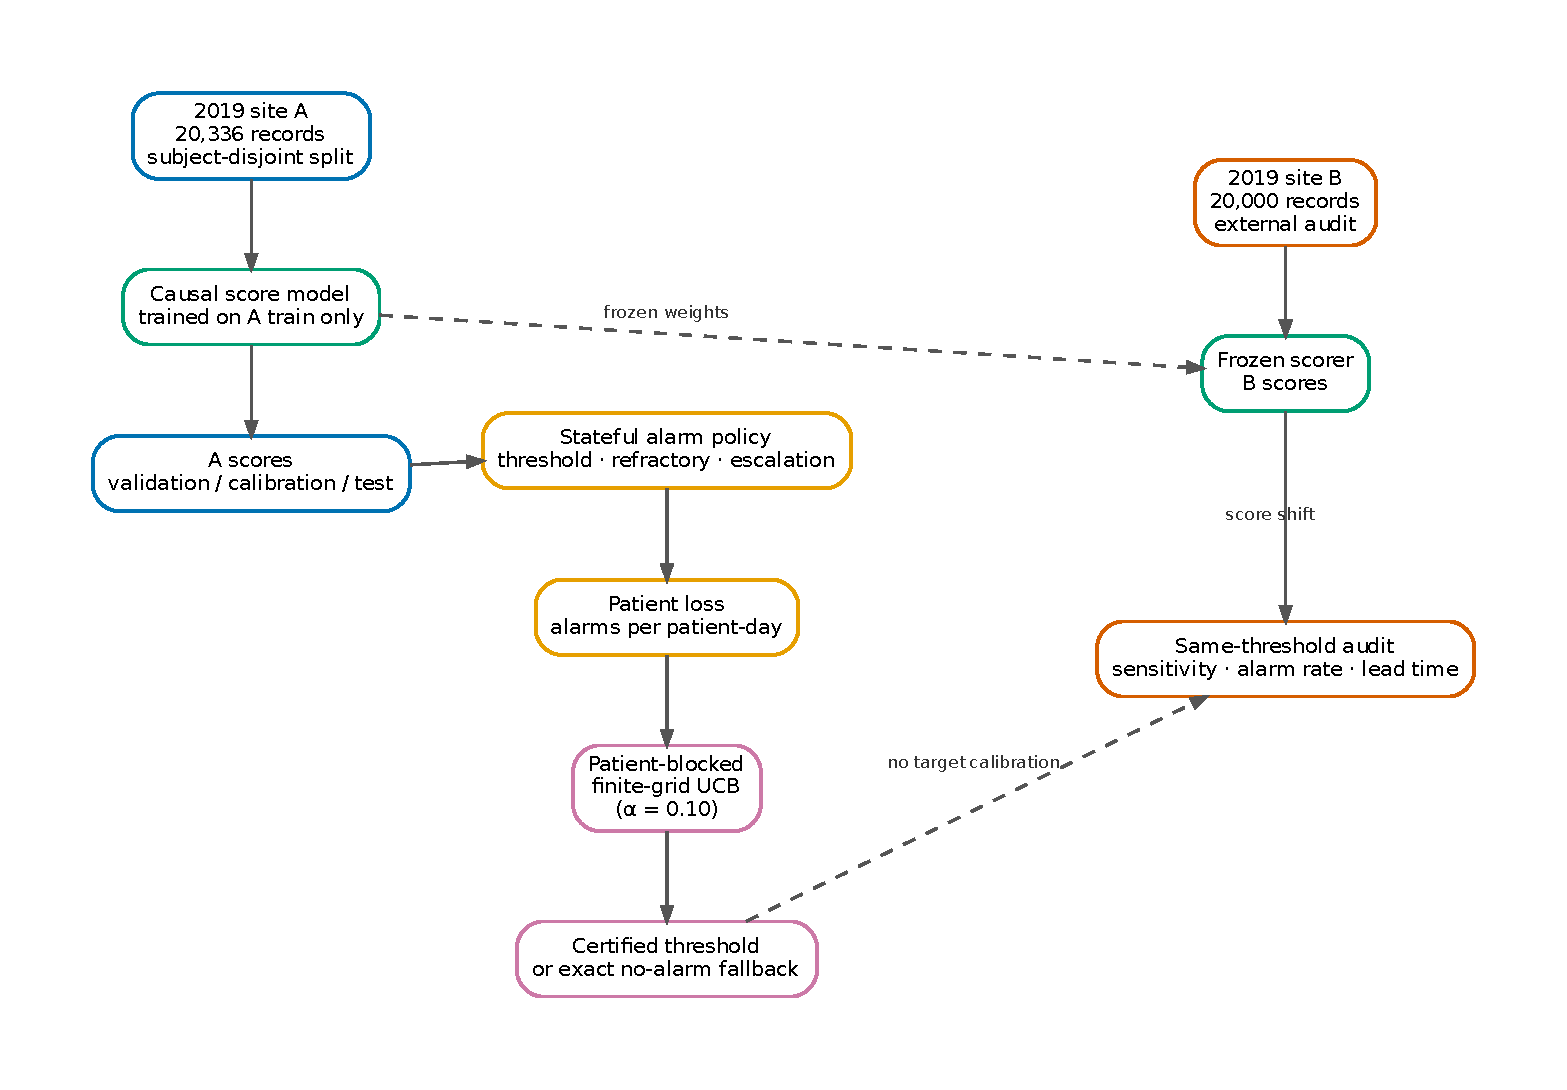
\includegraphics[width=\linewidth]{figures/framework.pdf}
\caption{Evaluation design. A causal score model is fitted on site A training records and frozen before site B is touched. The stateful policy replays each patient trajectory to obtain alarms per patient-day; a patient-blocked finite-grid upper confidence bound selects a threshold, or returns the exact no-alarm fallback when no candidate is certified. The primary external audit applies the same threshold without target-site calibration; the target-calibration diagnostic in the Results is a separate oracle analysis.}
\label{fig:framework}
\end{figure}

The audit also exposes substantial measurement heterogeneity. In site A, EtCO$_2$ is absent in every record, whereas 7.6\% of B records contain at least one EtCO$_2$ value; temperature is observed in only 33.8\% of A records, and several laboratory variables are observed in fewer than 5\%. This pattern motivates retaining a fixed variable set across sites and explicitly handling all-missing training columns, rather than fitting site-specific feature matrices. The 2012 mortality cohort \citep{citi2012physionet} was retained only as an ingestion and outcome-join check; because it has no deterioration onset, we do not treat its 49 decision points as a same-task external validation.

\subsection{Labels, Partitions and Eligibility}

The supplied 2019 label becomes positive six hours before the challenge-defined clinical onset. We set \texttt{label\_lead\_hours}$=6$ to recover the candidate clinical time and \texttt{horizon}$=6$ to label the six preceding hours positive. Timesteps at or after onset, padded steps, and all steps of a left-censored record are excluded from discrimination and calibration targets. An event at or beyond the end of observed follow-up is not counted as a detectable lead-time case.

The official 2019 release stores one PSV file per subject, and we use ``subject'' and ``patient'' interchangeably for this cohort. We use the file stem as the subject identifier and verify that every identifier occurs in exactly one partition; the split audit is written to the run metadata. For each random seed we use a subject-disjoint 60/15/10/15 split into training, validation, calibration and test subjects. The scorer, preprocessing, structural policy parameters and threshold grid are fixed using training and validation subjects. The calibration partition selects the deployed threshold, and the test partition is touched only for evaluation. Site B is evaluated with the A-trained scorer and the A-calibrated threshold; no B labels are used for target calibration. Three seeds (0, 1, 2) are reported for the prefix logistic model, the masked GRU, the LightGBM baseline and the E2 budget sweep. The target-site recalibration diagnostic is reported for all three logistic seeds and for one GRU seed, and is labelled as an oracle analysis throughout.

A separate target-site diagnostic asks how much of the external loss is recoverable when target labels are available. We split the eligible B subjects into disjoint calibration and test halves of equal size using a site-specific random permutation (seed $1000+s$ for source seed $s$), recalibrate the same policy family and threshold grid on B calibration subjects, and evaluate on B test subjects. This analysis uses target labels for threshold selection and is therefore an oracle-style target-calibrated reference estimate rather than a deployable label-free procedure; it is reported separately from the primary external audit and never used to tune the A model.

The target label-budget curve fixes the B test half and draws nested calibration subsets of 5\%, 10\%, 25\% and 50\% of all eligible B subjects from the remaining half. The same threshold selector is refitted on each subset and evaluated on the common test half, so the curve isolates calibration-set size. The source-threshold point is evaluated on the same test half and serves as the zero-label reference.

The support bound requires an independently declared minimum exposure. We use $H_{\min}=24$ hours, which retains 15{,}837 of 20{,}336 A records and 14{,}824 of 20{,}000 B records. This is an eligibility restriction, not a post-hoc filter chosen to improve results. Alarm-rate evaluation counts the full observed exposure, including time after onset; lead-time evaluation uses only the pre-onset window. With hourly decisions, refractory $\tau=4$ and no escalation, the resulting support bound is $L_{\max}=144/26\approx5.54$ alarms per patient-day.

\subsection{Score Models}

The primary scorer is a causal prefix-feature logistic regression. At each decision step it uses the last observed value of every variable, the cumulative observation fraction, and admission static features. All features are computed from current and past observations only. Median imputation is fitted on the training partition with empty features retained, so a variable that is entirely missing at site A remains a constant column at site B instead of silently changing the feature dimension. The classifier uses $C=1$ and a maximum of 2{,}000 iterations. A unidirectional masked GRU with 64 hidden units is used as a secondary architecture check. It consumes observed values, observation masks, log-transformed elapsed time and static features; it is a reference implementation, not a GRU-D reproduction. The GRU is trained for 20 epochs with Adam at $10^{-3}$, batch size 64, and a fixed random seed on an RTX 4090. A LightGBM gradient-boosted tree classifier is fitted to the same prefix features with 300 trees, learning rate 0.05, 31 leaves and median imputation; it is reported as a stronger tabular baseline, not as a tuned state-of-the-art model.

Partial NEWS, SIRS and qSOFA scores are computed from the variables available in the 2019 release, following the standard early-warning-score and instrument definitions \cite{price2023evaluating,candel2023development}. NEWS omits the consciousness and supplemental-oxygen components, SIRS omits the immature-neutrophil alternative, and qSOFA omits the Glasgow Coma Scale; these are research-only partial instruments, not certified clinical implementations. Charted observations are placed on the ICULOS clock, forward-filled, and scored per timestep. Steps before the first observed component are backfilled with the first finite score, and any remaining unobserved step receives zero points; this is a no-points convention, not an assertion that the patient was clinically normal. Their thresholds are calibrated on the same A calibration subjects at the same requested budgets as the learned scorers, so the comparison is a matched-workload audit rather than a claim that the instruments are equivalent.

\subsection{Alarm Policy and Calibration}

The policy family is the stateful rule in \cref{eq:policy}. We fix refractory $\tau=4$ decision steps, escalation $\kappa=0$, and a 12-hour lead window $W=12$. The candidate grid is 200 equally spaced thresholds from 0.01 to 0.99; the grid is fixed before calibration. The risk level is $\alpha=0.10$, and the reported certificates use the empirical-Bernstein radius in \cref{eq:bernstein}; Proposition~\ref{prop:eb} gives its finite-grid validity, while the Hoeffding radius in Proposition~\ref{prop:validity} is retained as the conservative variant. The selector deploys the smallest threshold whose raw empirical loss plus radius is at most the requested budget. If no threshold is certified, the exact no-alarm fallback is reported rather than silently substituting the largest finite threshold.

For each patient and threshold, the full stateful trajectory is replayed once to obtain alarms per patient-day. This loss matrix is reused across budgets and across the blocked and timestep procedures, so differences between procedures come only from the confidence radius and not from a different point estimator. The deliberately invalid timestep comparator substitutes calibration timesteps for calibration patients in the Hoeffding radius; it is a diagnostic, not a proposed method.

\subsection{Metrics and Uncertainty}

Discrimination is summarized by AUROC and AUPRC over usable pre-onset timesteps. Because the positive-timestep prevalence is only 1.27\% in the A test partition and 0.72\% at B, AUPRC is interpreted against that prevalence rather than against 0.5. Calibration is summarized by 10-bin expected calibration error (ECE); ECE is descriptive and does not establish clinical calibration. Operational metrics are the realised patient-average alarm rate, event sensitivity in the 12-hour lead window, median lead time among detected events, and the fraction of test patients whose per-day alarm count exceeds the requested budget.

Confidence intervals for score metrics use a patient-level bootstrap with 400 resamples, preserving within-patient dependence. Operational intervals use 2{,}000 patient-block resamples on seed 0 and resample whole target subjects, so within-subject alarm dependence is preserved; paired differences use the same resampled subjects and Holm correction across the reported comparisons. Two-sided bootstrap $p$-values are not a substitute for external validation. Operational curves report the mean and sample standard deviation over seeds; no interval is attached to the single-seed target-site GRU diagnostic.

\subsection{Reproducibility and Compute}

All raw records and score caches are kept outside the manuscript repository. The code exposes separate entry points for downloading and checksumming the 2019 release, auditing the official files, fitting and caching E1 scores, sweeping E2 budgets, bootstrap intervals and seed aggregation. The full test suite (135 tests) passes on the execution machine. The GRU uses CUDA but no formal GPU-hour or energy measurement was recorded; runtimes are therefore reported as implementation facts, not as a compute-efficiency claim.


% Sections below are written only after experiments are complete.
% \section{Results}
\label{sec:results}
\subsection{Cohort Audit and Score Discrimination}

The public cohort is large enough to estimate patient-level alarm rates, but its measurement process is far from uniform. Table~\ref{tab:cohort} shows that site A has a higher positive-record fraction than site B (8.8\% versus 5.7\%), while both sites contain a non-trivial number of left-censored records whose first label is already positive. The observed-variable table also explains why a naive cross-site model can fail: EtCO$_2$ is entirely absent at A but present in 7.6\% of B records, and temperature is observed in only about one third of either cohort. A model that drops an all-missing training column would therefore change its input dimension at the external site; the implementation retains such a column as a constant during imputation and the regression test in the repository checks this case explicitly.

\begin{table}[tb]
\centering
\caption{Public 2019 cohort audit after downloading and checksum verification. Percentages for observed variables are the fraction of records with at least one non-missing value. The two sites are separate hospital systems.}
\label{tab:cohort}
\begin{tabular}{lrr}
\toprule
Quantity & Site A & Site B \\
\midrule
Records & 20{,}336 & 20{,}000 \\
Positive records & 1{,}790 & 1{,}142 \\
Left-censored records & 203 & 223 \\
Identifiable pre-onset events & 1{,}587 & 919 \\
Median observed stay (h) & 39 & 38 \\
EtCO$_2$ observed (\%) & 0.0 & 7.6 \\
Temperature observed (\%) & 33.8 & 33.9 \\
Lactate observed (\%) & 3.4 & 1.9 \\
\bottomrule
\end{tabular}
\end{table}

Table~\ref{tab:discrimination} reports three-seed score discrimination. The prefix logistic model reaches an A-test AUROC of $0.736\pm0.013$ and AUPRC of $0.034\pm0.006$; the masked GRU reaches $0.743\pm0.011$ and $0.043\pm0.005$, and LightGBM reaches $0.763\pm0.009$ and $0.042\pm0.004$. These AUPRC values must be read against the 1.27\% positive-timestep prevalence: both models rank positive steps several times better than chance, but the absolute positive predictive signal remains modest. On site B the logistic model falls to $0.676\pm0.005$ AUROC and $0.017\pm0.000$ AUPRC, while the GRU reaches $0.683\pm0.004$ and $0.018\pm0.002$, and LightGBM reaches $0.713\pm0.003$ and $0.025\pm0.001$. Ten-bin ECE is small in absolute terms (0.0011 and 0.0017 at A; 0.0014 and 0.0018 at B), but it is descriptive and should not be read as evidence of clinical calibration under shift. The drop is consistent with multisite sepsis-model evaluations that report degraded transport across hospitals \citep{valan2025evaluating,ostermayer2024external}, and it is larger in AUPRC than in AUROC because prevalence also changes.

\begin{table}[tb]
\centering
\caption{Three-seed score discrimination (mean $\pm$ sample standard deviation). AUPRC is computed over usable pre-onset timesteps; positive-timestep prevalence is 1.27\% at A and 0.72\% at B. Ten-bin ECE is reported in the text and is descriptive.}
\label{tab:discrimination}
\small
\begin{tabular}{lcccc}
\toprule
 & \multicolumn{2}{c}{Site A test} & \multicolumn{2}{c}{Site B external} \\
\cmidrule(lr){2-3}\cmidrule(lr){4-5}
Model & AUROC & AUPRC & AUROC & AUPRC \\
\midrule
Prefix logistic & $0.736\pm0.013$ & $0.034\pm0.006$ & $0.676\pm0.005$ & $0.0172\pm0.0002$ \\
Masked GRU & $0.743\pm0.011$ & $0.043\pm0.005$ & $0.683\pm0.004$ & $0.0183\pm0.0016$ \\
LightGBM & $0.763\pm0.009$ & $0.042\pm0.004$ & $0.713\pm0.003$ & $0.0250\pm0.0010$ \\
\bottomrule
\end{tabular}
\end{table}

The seed-0 patient bootstrap sharpens the comparison without turning a small numerical difference into a claim. At site A the logistic model has AUROC $0.741$ with 95\% interval $[0.710,0.766]$ and AUPRC $0.041$ with interval $[0.035,0.051]$; the GRU has AUROC $0.744$ $[0.716,0.772]$ and AUPRC $0.044$ $[0.038,0.056]$. The paired GRU-minus-logistic difference is $0.004$ for AUROC with interval $[-0.023,0.032]$ and two-sided $p=0.775$, and $0.003$ for AUPRC with interval $[-0.006,0.014]$ and $p=0.42$. The GRU is therefore a secondary architecture check, not a demonstrated improvement. At site B the AUROC difference is essentially zero, while the AUPRC difference is $0.003$ with interval $[0.0002,0.0059]$ and $p=0.05$; this isolated interval is reported as exploratory because it is not corrected across metrics or sites.

\subsection{Budgeted Alarm Policies and Cross-Site Transport}

Figure~\ref{fig:budget} and Table~\ref{tab:e2} report the operational frontier for the prefix logistic scorer. On site A, raising the requested budget from 0.25 to 2 alarms per patient-day increases mean sensitivity from $0.185\pm0.061$ to $0.774\pm0.032$, while the realised alarm rate rises from $0.108\pm0.012$ to $1.366\pm0.026$. The realised rate stays below the requested budget at every operating point, which is the expected consequence of a finite-sample upper bound rather than evidence that the policy is slack by design. The tightest budget has the largest seed-to-seed sensitivity variance, because a small change in the calibrated threshold moves several of the 168 eligible A events across the detection boundary. Median lead time among detected events stays between 8.7 and 10 hours, but this conditional median must be read with the corresponding sensitivity: it describes only the events that were detected.

\begin{figure}[tb]
\centering
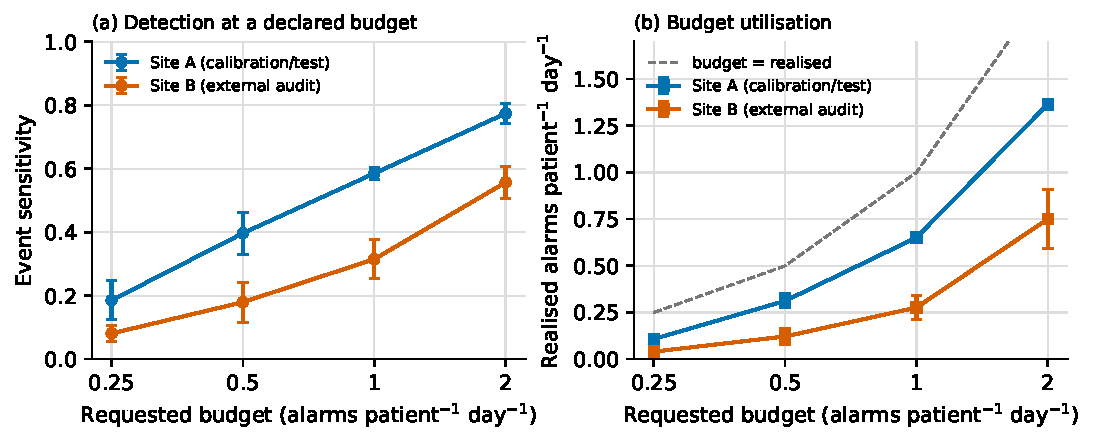
\includegraphics[width=\linewidth]{figures/e2_budget.pdf}
\caption{Three-seed E2 operating curves for the prefix logistic scorer. (a) Event sensitivity versus the requested patient-average alarm budget. (b) Realised alarm rate versus the requested budget; the dashed diagonal marks exact budget utilisation. Error bars are sample standard deviations over seeds 0--2. Site B uses the A-calibrated threshold without target labels.}
\label{fig:budget}
\end{figure}

\begin{table}[tb]
\centering
\caption{E2 budget sweep for the prefix logistic scorer, mean $\pm$ sample standard deviation over three seeds. Rates are alarms per patient-day; lead time is the median among detected events in hours; violation is the fraction of test patients whose per-day count exceeds the budget. The 4- and 8-per-day rows coincide because the threshold grid reaches its floor.}
\label{tab:e2}
\small
\begin{tabular}{lcccc}
\toprule
\multicolumn{5}{c}{Site A (calibration/test)} \\
Budget & Rate & Sens. & Lead & Viol. \\
\midrule
0.25 & $0.108\pm0.012$ & $0.185\pm0.061$ & $9.5\pm0.5$ & $0.074\pm0.001$ \\
0.50 & $0.312\pm0.037$ & $0.397\pm0.067$ & $8.7\pm0.6$ & $0.151\pm0.014$ \\
1.00 & $0.651\pm0.022$ & $0.585\pm0.020$ & $9.3\pm0.6$ & $0.210\pm0.003$ \\
2.00 & $1.366\pm0.026$ & $0.774\pm0.032$ & $10.0\pm0.0$ & $0.309\pm0.004$ \\
4.00 & $2.096\pm0.026$ & $0.894\pm0.011$ & $10.0\pm0.0$ & $0.271\pm0.012$ \\
\bottomrule
\end{tabular}

\vspace{6pt}
\begin{tabular}{lcccc}
\toprule
\multicolumn{5}{c}{Site B (external audit)} \\
Budget & Rate & Sens. & Lead & Viol. \\
\midrule
0.25 & $0.040\pm0.014$ & $0.081\pm0.026$ & $8.5\pm0.5$ & $0.030\pm0.010$ \\
0.50 & $0.122\pm0.044$ & $0.180\pm0.063$ & $8.2\pm0.3$ & $0.065\pm0.023$ \\
1.00 & $0.276\pm0.063$ & $0.315\pm0.062$ & $8.3\pm0.6$ & $0.094\pm0.025$ \\
2.00 & $0.750\pm0.157$ & $0.557\pm0.051$ & $9.0\pm0.0$ & $0.163\pm0.038$ \\
4.00 & $1.473\pm0.250$ & $0.724\pm0.049$ & $9.3\pm0.6$ & $0.131\pm0.025$ \\
\bottomrule
\end{tabular}
\end{table}

The external audit exposes a qualitatively different operating point. At the 1-per-day budget the A-calibrated policy emits $0.276\pm0.063$ alarms per B patient-day, less than half the A rate, and detects $0.315\pm0.062$ of eligible B events compared with $0.585\pm0.020$ at A. At the tightest budget, B sensitivity falls to $0.081\pm0.026$ while the realised B alarm rate is only $0.040\pm0.014$. The direction of the rate change is not a free lunch: the same threshold is simply less active on the shifted score distribution, and the lost activity is concentrated on true events. This is exactly the failure mode that a threshold-only transport claim would hide, and it is consistent with recent evidence that score distributions and calibration can shift across hospitals \citep{lu2022estimating,wu2026outofdistribution}. A target-site calibration study is therefore a separate deployment step, not an optional refinement.

The deliberately invalid timestep comparator is less conservative at the two tightest budgets. At budget 0.25 it selects threshold 0.0445 instead of 0.0543, raises the A alarm rate from 0.117 to 0.183, raises A sensitivity from 0.250 to 0.321, and raises the patient-violation fraction from 0.074 to 0.115. At budget 0.50 it selects 0.0297 instead of 0.0346, raises the alarm rate from 0.328 to 0.450, raises sensitivity from 0.452 to 0.512, and raises the violation fraction from 0.161 to 0.214. At budgets of 1 and above the finite grid selects the same threshold for both procedures on this split, so the comparator is not a universal ranking. The result is nevertheless the expected qualitative signature of effective-sample-size inflation: the timestep procedure buys sensitivity by shrinking its guard band and paying for it in per-patient budget violations.

The GRU changes the level of the frontier but not its transport behaviour. At 1 alarm per patient-day its seed-0 A sensitivity is 0.685 and its B sensitivity is 0.326, compared with 0.607 and 0.382 for the logistic model. At 0.25 per day the GRU reaches 0.393 at A and 0.129 at B. The GRU therefore looks better than logistic at the tight internal budget and at the moderate internal budget, but worse at the external 1-per-day point; the ordering is not stable across sites. This is a useful negative result for architecture-centred claims: a more expressive scorer can move the internal frontier without repairing the site shift. It also reinforces that the calibration procedure, not the backbone alone, determines whether a stated alert budget is met.

Two limitations of the grid are visible in the table. First, the 4- and 8-per-day rows are identical because the threshold grid stops at 0.01; above roughly 2 alarms per patient-day the budget constraint is no longer binding and the frontier is truncated by the candidate set. Second, every certified operating point has a realised rate below its requested budget, so the experiment demonstrates conservative risk control rather than tight budget utilisation. Neither observation undermines the certificate, but both matter for engineering deployment: a hospital that needs a precise alarm load may prefer a finer grid or a utility-based selection among certified thresholds, and a hospital that needs a higher sensitivity must accept the corresponding increase in realised alert volume. The clinical interpretation of these rates also depends on local workflow and alarm-fatigue tolerance, which this retrospective study does not measure \citep{ray2026alert,jaidev2026sepsis}.


% \section{Discussion}
\label{sec:discussion}

The central empirical finding is that a patient-blocked alarm budget is portable as a \emph{constraint} but not as a \emph{threshold}. Within site A, the calibrated policy moves smoothly from 0.19 sensitivity at 0.25 alarms per patient-day to 0.77 at 2 per day, and the realised rates remain below the requested budgets. When the same A-calibrated threshold is applied to site B, the realised rate falls to roughly half the A rate and sensitivity at 1 per day falls from 0.585 to 0.315. The budget itself is still respected in the sense that B's realised mean is below the A certificate, but the clinical yield is much lower. This distinction matters for engineering practice: a site that imports only a threshold has not imported the operating point that the source site validated.

The comparison with the timestep shortcut clarifies what patient blocking buys. At the tightest budgets the timestep procedure selects a lower threshold and increases both sensitivity and the fraction of patients exceeding the budget. That is a real trade, not a statistical technicality: the method that treats correlated hours as independent observations is more willing to spend a fixed nominal risk budget, and the additional alarms are not free at the patient level. At looser budgets the finite grid collapses the two procedures to the same threshold, so the experiment should not be read as a claim that timestep calibration always fails. The defensible conclusion is narrower and stronger: when the estimand is a patient-average rate, the effective sample size is the number of independent patients, and methods that substitute timesteps can become less conservative without a corresponding patient-level guarantee.

The backbone comparison is more nuanced than a single ranking. LightGBM has the highest site-B AUROC ($0.713\pm0.003$) and the highest external sensitivity at 1 per day ($0.540\pm0.071$), while the GRU has the highest site-A sensitivity ($0.684\pm0.006$) and LightGBM is second ($0.661\pm0.042$). The seed-0 paired LightGBM-minus-logistic sensitivity difference at B is $0.081$ with interval $[0.027,0.133]$ and Holm-adjusted $p=0.066$, whereas the GRU-minus-logistic difference is $-0.056$ with an interval that includes zero after Holm adjustment. A stronger tabular scorer therefore narrows the external gap, but it does not remove the transport problem: LightGBM's B rate is $0.410\pm0.156$, still below the requested 1 per day, and the target label-budget analysis shows that local labels remain necessary to move the operating point. This is consistent with the broader observation that clinical prediction performance is often more sensitive to cohort and workflow differences than to modest architecture changes \citep{valan2025evaluating,ostermayer2024external,wu2026outofdistribution}. It also argues against presenting a backbone-only AUROC table as evidence of deployability.

For engineering deployment, the results support four concrete practices. First, the minimum observed stay used in the support bound should be declared before looking at calibration or test outcomes, because it changes both eligibility and $L_{\max}$; the 24-hour restriction here removes about 22\% of A records and 26\% of B records. Second, the no-alarm fallback should remain an explicit, auditable state rather than being replaced by the largest finite threshold, since the latter can still alarm and has no certificate. Third, a target site that has local labels should recalibrate on its own patient blocks before adopting a source threshold, because the external rate and sensitivity can move in opposite directions; our oracle split shows that this recovers part of the sensitivity but not without a higher alarm load, and a label-free version remains an open deployment problem. Fourth, the threshold grid and the realised-rate report should be published together, since a grid floor can make high budgets look identical and hide the fact that the constraint is no longer binding. These practices are operational rather than architectural, and they are compatible with the alert-stewardship literature that treats interruptive alerts as a monitored resource \citep{khan2026qualitative,ray2026alert,jaidev2026sepsis}.

The study has several limitations that bound its claims. It is retrospective and uses a single public challenge cohort with two sites; the subject-disjoint split uses the official one-file-per-subject structure, but the release cannot link separate readmissions, so the independent-subject assumption remains an assumption. The label is the challenge's sepsis definition, not a adjudicated clinical deterioration event, and left-censored records are excluded rather than imputed. The score models are deliberately simple reference learners, LightGBM is not tuned, and the GRU is not a state-of-the-art architecture. The partial NEWS, SIRS and qSOFA baselines omit components that the 2019 release does not contain, so they are research comparators rather than certified clinical instruments. No label-free target-site adaptation, subgroup analysis, observation-sparsification study or clinical outcome evaluation was performed; the target-site recalibration and label-budget analyses are oracle diagnostics that use target labels and are not deployment procedures. ECE is low in absolute terms but is computed on a low-prevalence timestep problem and should not be read as clinical calibration. The primary external evaluation has no B calibration set by design, so it measures transport failure rather than the best achievable B performance. The three-seed E2 comparison is complete for all three backbones, but the target-site diagnostic for the GRU is single-seed, the label-budget curve is conditional on one target split and one policy family, and the study does not estimate GPU-hours or alert-fatigue outcomes.

These limitations do not overturn the methodological result, but they change what should be claimed. The paper does not show that budgeted calibration improves patient outcomes, reduces mortality or is preferred by clinicians. It shows that a stateful policy can be calibrated against a patient-level alarm budget with a finite-sample bound, that the resulting operating curve is measurable on a public cohort, and that the same threshold does not transport unchanged across hospitals. That is a narrower contribution than a clinical-effectiveness claim, but it is a more honest one, and it identifies the target-calibration experiment that a deployment study would need to run next.

% \section{Conclusion}
\label{sec:conclusion}

This paper treated early warning as a stateful alarm policy whose alert load is a declared design constraint rather than an emergent threshold artefact. We derived a patient-blocked finite-grid upper-confidence procedure for the population mean of patient-level alarms per day, separated it from a deliberately invalid timestep effective-sample-size shortcut, and implemented the complete path from causal scoring through policy replay to auditable operating points. On the public 2019 A/B cohort, the procedure produced a monotone internal budget-sensitivity frontier, with A sensitivity rising from 0.185 at 0.25 alarms per patient-day to 0.774 at 2 per day over three seeds. The same A-calibrated threshold did not transport to site B: at the 1-per-day budget, B sensitivity was 0.315 versus 0.585 at A, even though the realised B alarm rate remained below the A certificate. An oracle target-site recalibration raised B sensitivity to 0.497 but also raised the realised rate to 0.616, and a nested label-budget analysis showed that roughly 10\% of the eligible target subjects (about 1,482 patients) recovered the full-pool threshold at 1 per day while 5\% remained unstable across seeds. LightGBM raised B sensitivity at 1 per day to 0.540 and the GRU reached 0.375, but neither removed the cross-site shift; the timestep comparator was less conservative at tight budgets and increased patient-level budget violations. These results support budgeted, patient-blocked calibration as an engineering instrument, but they do not establish clinical effectiveness, alert-fatigue reduction or deployment readiness; label-free target adaptation, subgroup and missingness analyses, prospective outcome evaluation and a finer utility-aware grid remain necessary before any clinical claim.


\FloatBarrier
\bibliographystyle{elsarticle-num}
\bibliography{refs}

\end{document}
